% First release on June 21, 2010
% Modified on Dec 12, 2017 by XSK

\documentclass[twoside,twocolumn]{article}
\def\@oddhead{\mbox{}\scriptsize\rightmark \hfil \thepage}%
\usepackage{fitee}
\usepackage{tabularx, multirow}
\usepackage{graphicx}
\usepackage{subfigure}
%\usepackage[colorlinks, breaklinks = true]{hyperref}		% for pdflatex
\usepackage[dvips, hidelinks, breaklinks = true]{hyperref}  % for DVI to PDF latex
\newcommand{\todo}[1]{\textcolor{red}{\textbf{#1}}}
\addto{\captionsenglish}{%
  \renewcommand{\figurename}{Fig.}
}

%\usepackage[labelformat=simple,font=footnotesize]{subcaption}
%\renewcommand\thesubfigure{(\alph{subfigure})}	% Put parens around subfig ref

\begin{document}

%% article title
\title{Improving Neighbor Discovery with Slot Index Synchronization}

%% when all authors provide emails, no $\dagger$
\author[$\dagger$$\ddagger$1]{Shuai-zhao JIN}%
\author[$$2]{Zi-xiao WANG}%
%\author[$$2]{Ben Leong}%
\author[$$1]{Ya-bo Dong}%
\author[$$1]{Dong-ming Lu}
\affil[1]{School of Computer Science and Technology of Zhejiang University, Hangzhou 310027, China}
\affil[2]{Department of Computer Science, National University of Singapore, Singapore}

\shortauthor{Jin et al.}	% one author: only Zhai; two authors: Zhai and Hu; three authors: Zhai et al.

\authmark{}

%% Only 1 affiliations
%\author{Wen-fei WANG}
%\author{Rong XIONG$^{\dagger\ddagger}$}
%\author{Jian CHU}
%\affil{\it\footnotesize State Key Laboratory of Industrial Control Technology, Institute of Cyber-Systems and Control,
%	\authorcr\it\footnotesize Zhejiang University, Hangzhou 310027, China}

% for authors, use \authorcr to begin with a new line, e.g., \author[2]{\authorcr Xian-liang HU}
% for the affiliation, use \authorcr\Affilfont\it to begin with a new line, e.g.,
%\affil[1]{Editorial Office of Journal of Zhejiang University SCIENCE,
%\authorcr\Affilfont\it Hangzhou 310027, China}

\corremailA{jinszhao@zju.edu.cn} 
%\corremailB{xlhu@zju.edu.cn}
%\corremailC{abc@zju.edu.cn}
%\corremailD{ABC@zju.edu.cn}
\emailmark{$\dagger$}	% when all authors provide emails, no \dagger


% abbrev. of month: Jan. Feb. Mar. Apr. May June July Aug. Sept. Oct. Nov. Dec.
\dateinfo{Received mmm.\ dd, 2016;	Revision accepted mmm.\ dd, 2016;    Crosschecked mmm.\ dd, 2017}


\abstract{Neighbor discovery is important for \emph{docking} applications, where mobile nodes communicate with
static nodes situated at various rendezvous points. Among existing neighbor discovery protocols, probabilistic
methods perform well in the average case but have aperiodic, unpredictable and unbounded discovery latency.
While deterministic protocols can provide a bounded worst-case discovery latency, they achieve this by
sacrificing the average-case performance. In this paper, we propose Mobility-Assisted Slot index Synchronization
(MASS), a new synchronization technique that improves the average-case performance of deterministic
neighbor discovery protocols via \emph{slot index synchronization}, without incurring additional energy consumption.
We evaluate MASS through both theoretical analysis and simualtions of real traces from a tourist tracking system
deployed at Mogao Grottoes, a famous cultural heritage site in China. We show that MASS can reduce the average
discovery latency of state-of-the-art deterministic neighbor discovery protocols by up to 2 orders of magnitude.
}
% separate by semicolons 
\keywords{Neighbor discovery; Docking applications, Slot index synchronization; MASS}


\doi{10.1631/FITEE.1000000}	% DOI of the paper, should be accurate
\code{A}
\clc{TP}

%\inpress	% uncomment this command if use "in press"

\publishyear{2018}
\vol{19}
\issue{1}
\pagestart{1}
\pageend{5}

%% when no funding, the following line should be removed, no period at last
\support{Project supported by the National High Technology Research and Development Program of China (No.2012AA101701) and
the National Key Technology Support Program of China (No.2013BAK01B00, No.2014BAK16B00)} 

%\conf{A preliminary version of this paper has been presented at ??? Conference, date}
%\esm{Electronic supplementary materials: The online version of this article (http://dx/doi.org/10.1631/jzus.C1000000) contains supplementary materials, which are available to authorized users}
\orcid{Shuai-zhao JIN, http://orcid.org/0000-0002-5176-5607}	% corresponding author, or first author
\articleType{}
%\articleType can be `Science Letters:', `Review:', `Comment:', etc.
%Leave blank for research article.

\maketitle



\section{Introduction} 
\label{sec:introduction}
The availability of cheap wireless sensor nodes has made \emph{docking} applications~\citep{Dutta2008Practical} 
feasible for widespread deployment. In docking applications, there are two sets of sensor nodes: static and mobile
nodes. Static nodes are placed at fixed rendezvous points and mobile nodes are attached to moving objects of interest.
Some examples of docking applications include the uploading of cargo transit history~\citep{malinowski2007cargonet}, 
cattle movement tracking during feeding times~\citep{wark2007model}, hikers tracking via their encounters 
with trail-sid waypoints~\citep{huang2005cenwits} and tourist tracking, which tracks tourists at a cultural heritage 
site~\citep{ming2008wireless}.

For the conservation work in Mogao Grottoes, a famous cultural heritage site in China, it is essential to track and 
study how the movement of tourists around the caves affects the microclimate in caves. The current tracking system
in place consists of static nodes placed in the caves and mobile nodes carried by the tour guides. The static nodes
emit beacons which are picked up by the mobile nodes for each tour group that enters a cave. Not only is the 
detection of the tour group important, it is also essential to accurately measure the duration of stay within each
cave. In addition, power is also a constraint for the tracking system as modern infrastructure is not allowed to be
installed in the caves to supply power to the static nodes.

In the current tracking system, the static nodes are configured at a duty cycle of 0.6\%~(they wake up and send beacons
for 30~ms every 5~s) and the mobile nodes are always active and continuously listen for the beacons. While this achieves
an average discovery latency of 2.5~s, the mobile nodes have to be charged daily, which is inconvenient and is also a
major impediment to our plans for scaling up the system. Our goal is to reduce energy consumption by introducing duty
cycling for the mobile nodes, without compromising discovery latency.

Neighbor discovery protocols will allow both the static and mobile nodes to duty cycle while ensuring discovery. Through
different wake-sleep patterns design, neighbor discovery protocols ensure that nodes will wake up within the same time
slot to discover each other. Our key insight is that \emph{discovery latency can be minimized by synchronizing the active 
and sleeping slots of the nodes}. This is because when the slot indices are synchronized, the nodes will discover each 
other at the next earliest active slot, i.e., the next overlapping active slot.

While this might sound straightforward, it turns out that synchronizing the nodes for a docking application introduces
a number of challenges. First, the synchronization must be done in a distributed manner as the static nodes cannot 
directly communicate with each other. Instead, they can only communicate by using the mobile nodes to relay information,
 i.e., mobiles nodes work as proxy. Second, the synchronization should converge quickly in order to achieve any gains. 
Finally, the intrinsic inaccuracies in the clocks of the sensors will result in \emph{clock drift}. If the synchronization 
of the slots drifts by a small amount, the resulting latency could potentially become the worst case, instead of being optimal. 
In other words, synchronization could significantly degrade performance instead of improving performance if we are not careful.

We propose and evaluate Mobility-Assisted Slot index Synchronization~(MASS), which improves the average-case performance
of existing deterministic neighbor discovery protocols via \emph{slot index synchronization}. In MASS, the nodes first
elect a reference node in a distributed manner and then synchronize their slot indices with that reference node. We
exploited the natural visiting patterns of tourists to elect the reference node. For our Mogao Grottoes traces, MASS is
able to synchronize all the 60 static nodes within three hours, which is less than half of the 10-hour operational period
of the site. But even if it is not able to synchronize all the nodes, we can still reduce the discovery latency for the
nodes that are synchronized. To mitigate the impact of the clock drift, MASS employs existing techniques to estimate the 
clock skew between the nodes and compensate for the clock drift with respect to the elected reference node. The experiments
show that our sensor nodes can achieve the error of 0.98~ms and 2.4~ms per hour for 50\% and 90\% of the time, respectively,
which is well within one slot interval.

We evaluate MASS via simulation using a real 31-day trace obtained from the existing Mogao Grottoes tourist tracking system
and show that MASS can reduce the discovery latency of 4 existing deterministic protocols~(BlindDate~\citep{wang13blinddate}, 
Searchlight~\citep{bakht2012searchlight}, Disco~\citep{Dutta2008Practical} and U-Connect~\citep{kandhalu2010u}) by about 2 
orders of magnitude over 75\% of the time. Therefore, with MASS, we are able to achieve a discovery latency of less than 5~s
for 70\% of the time, even when the duty cycle of the nodes is reduced to 0.5\% to save power. By reducing the duty cycle
from 100\% to 0.5\%, our mobile nodes will be able to last 200 times longer and be charged every 6 months instead of daily.

To the best of our knowledge, we are the first to propose the use of slot index synchronization to improve neighbor discovery
latency in docking applications. We addressed the resulting challenges by utilizing existing techniques such as clock skew
estimation and clock drift compensation, and proposing a synchronization process and priority metric. It remains as future
work to thoroughly investigate how MASS performs on practical sensor networks, especially on the tourist tracking system
deployed at the Mogao Grottoes.

The rest of the paper is organized as follows: in Section~\ref{sec:related}, we present an overview of existing neighbor 
discovery protocols as well as clock synchronization and drift compensation techniques. In Section~\ref{sec:challenge}, 
we describe our docking application scenario, our key insight and explain the challenges for our system. In Section~\ref{sec:mass}, 
we describe the MASS algorithm. We evaluate MASS through a custom simulator in Section~\ref{sec:eval} and experiments in
a mock-up scenario in Section~\ref{sec:mock-up}. We conclude the paper in Section~\ref{sec:conclusion}.

\section{Related Work}
\label{sec:related}

{\bf Neighbor Discovery Protocols.} Neighbor discovery protocols are needed in duty-cycled 
networks to ensure discovery. Most neighbor discovery protocols are \emph{slotted} protocols
and divide time into identically-sized discrete slots. In each slot, sensor nodes either
sleep or wake up according to some pattern determined by the protocol. During \emph{active}
slots, the nodes wake up to transmit and listen for beacons from potential neighbors.
Existing protocols can be classified by their adoption of either \emph{probabilistic} or 
\emph{deterministic} wake-sleep slot schedules to achieve an overlap. In probabilistic 
protocols, the sleep-wake schedule is based on some randomized function~\citep{mcglynn2001birthday}. 
Generally, probabilistic protocols can achieve good average-case performance. Unfortunately, 
the worst-case performance is unbounded, i.e., there is a small chance that two nodes will 
never discover each other.

On the other hand, deterministic protocols provide a bounded worst-case latency as the sleep-wake 
schedule is designed to ensure discovery within one sleep-wake period. Prime-based protocols such 
as Disco~\citep{Dutta2008Practical} and U-Connect~\citep{kandhalu2010u} guarantee a bounded discovery 
latency based on the Chinese Remainder Theorem~\citep{niven2008introduction}. Quorum-based 
deterministic protocols~\citep{tseng2003power,lai2010heterogenous} have slots that are grouped into 
a 2-dimensional $m \times m$ array for a period of $m^2$.  Each node picks one row and one column 
of the entries as its active slots, thus ensuring that any two nodes will have at least two overlapping 
active slots in each period. The state-of-the-art Searchlight~\citep{bakht2012searchlight} protocol 
further reduces the overlapping slots to at least one by grouping the slots into an array of size 
$\lfloor\frac{m}{2}\rfloor \times m$. The duty cycle can be further reduced by {\em striped probing}, 
where the probe skips every two slots. Extending the duration of the active slots ensures overlap
and guarantees detection.  BlindDate~\citep{wang13blinddate} is a recently proposed protocol to 
improve the performance of Searchlight by having two dynamic probe slots traversing towards each other 
in opposite directions within each period. BlindDate also requires the extension of active slots like 
Searchlight.  Sun et al.\ proposed Hello~\citep{sun14hello}, a generalized framework for deterministic
protocols that can represent existing protocols such as Quorum, Disco, U-Connect and Searchlight, using 
a set of parameters.  They proved that Searchlight is the optimal symmetric protocol. Our technique,
MASS, complements existing deterministic protocols and can significantly reduce discovery latency 
through slot index synchronization.

{\bf Clock Synchronization.} There are two common approaches for clock synchronization in multihop 
wireless networks~\citep{sun14survey}: (i) reference-based clock synchronization; and (ii) distributed 
clock synchronization. In reference-based clock synchronization, the nodes synchronize their clocks 
with respect to one or more reference nodes. These reference nodes are known as roots in tree-based
protocols~\citep{su2005time,ganeriwal2003timing}, gateways in cluster-based protocols~\citep{elson2002fine}, 
and time servers in NTP-based protocols~\citep{ye2008dtp}. The main drawback of reference-based protocols 
is that they are not robust to the failures of reference nodes. Furthermore, they all assume that a 
reliable means of communication exists between the nodes.  This assumption does not hold for our tourist 
tracking system.

In distributed clock synchronization, all nodes run the same distributed synchronization algorithm, which 
will cause their local clocks to converge to a common global time value.  Some techniques to achieve global 
synchronization include having each node advance its clock to the fastest clock~\citep{jiang2004clock,zhou2007accurate}, 
or to the average clock values of the local nodes~\citep{li2006global,sommer2009gradient,sasabe2009simple}.  
Glossy is a recent network flooding architecture that achieves an average time synchronization error below 
one microsecond~\citep{ferrari11glossy}.  However, it is not suitable in docking applications because the 
mobile nodes are not always connected.  To cope with frequent topology changes and long inter-contact duration, 
Choi et al.\ developed distributed asynchronous clock synchronization (DCS) for delay tolerant networks~\citep{choi2012dcs}.  
Global clock synchronization is achieved by asynchronously compensating for clock errors using relative clock
information exchanged among nodes in DCS. The drawback of distributed synchronization algorithms is that 
convergence is slow (it typically takes hundreds of iterations)~\citep{he12random}. Furthermore, such
protocols only work well in a closed system, where no new nodes join the network once it starts.

\section{A Case for Slot Index Synchronization}
\label{sec:challenge}
In this section, we introduce the background for our target docking application system, 
and show that slot index synchronization is a promising technique to improve the 
performance of deterministic neighbor discovery protocols. We also explain why distributed
synchronization algorithms are not feasible for our application.

\subsection{Tourist Tracking in Historical Sites}

\begin{figure}[t]
  \centering 
  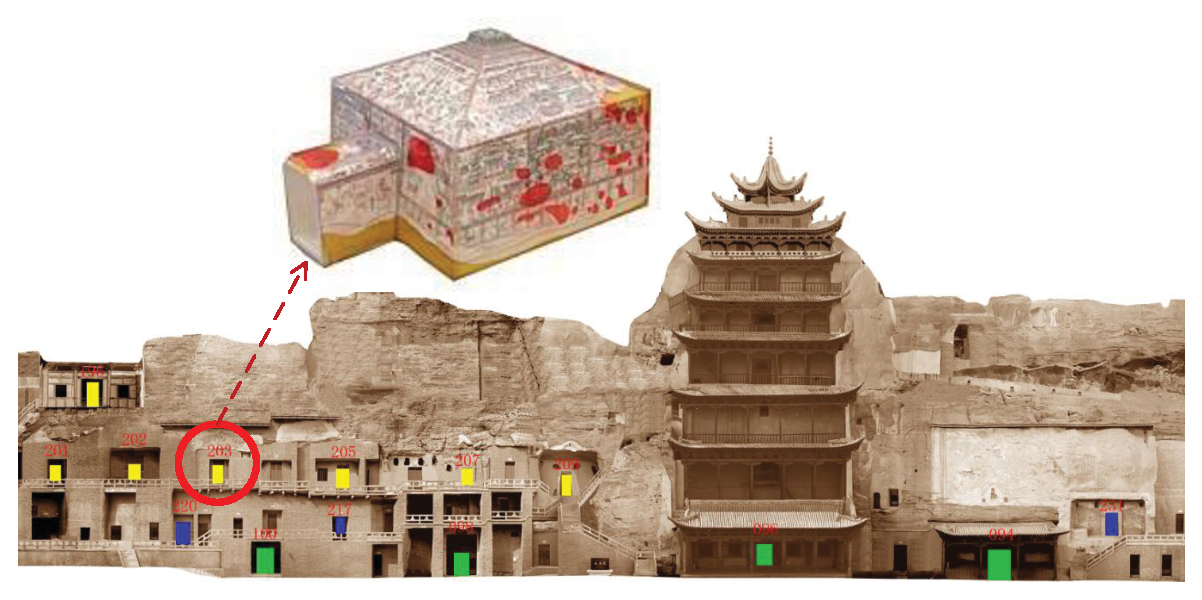
\includegraphics[scale=0.35]{static/mogao}
  \caption{A small section of Mogao Grottoes}
  \label{fig:mogao}
\end{figure}

Mogao Grottoes, also known as the Caves of the Thousand Buddhas, is a
famous cultural heritage site in China. It consists of hundreds of
caves cut into the side of a cliff, some of which have Buddhist murals
painted all over the walls and ceilings.  Fig.~\ref{fig:mogao} shows
a small section of the Mogao Grottoes. Thousands of tourists visit the
Mogao Grottoes every day, and the high volume of human traffic will
change the microclimate in caves which may cause deterioration to the 
priceless historical artwork. Therefore, it is important to monitor and 
limit the number of visitors to each cave to mitigate the over-exposure 
of the artwork due to human contact.

The challenge of tracking tourists in such a historical site is that
modern infrastructure such as power supply lines cannot be installed. 
Neither are fixtures allowed to be drilled into the walls
for fear of damaging the cultural artefacts. The current tracking
system deployed uses static low-power sensor nodes placed at the
corners of the caves which periodically emit beacon signals.  Each
tour guide holds a mobile sensor node that continuously listens for
and logs these beacons as the tour group visits each cave.  At the end
of the tour, the durations of the stay for each tour group in the
caves is extracted and recorded from the mobile nodes.

The tourist tracking system is an example of a {\em docking}
application. As the cave walls block the radio signals, static nodes
cannot communicate with each other directly. It is also not feasible
to deploy more nodes to create a fully connected wireless sensor
network due to conservation restrictions on the number of nodes that
can be deployed.

The lack of power infrastructure also means that static nodes have to
be powered by battery, which implies that energy consumption is a very
important consideration. To reduce energy consumption, the static
nodes currently perform duty cycle where they spend 30\,ms every 5\,s
listening and broadcasting beacons.  On the other hand, the mobile
nodes have to be continuously listening to detect static nodes as well
as record the entering and leaving time of tourists, thereby requiring
daily battery recharging. Considering hundreds of mobile nodes in use,
daily battery recharing is a huge impediment to scale up our tracking
system.

Neighbor discovery protocols provide a way to allow both the static and 
mobile nodes to duty cycle and thus reducing energy consumption. However, 
it is at the cost of increased discovery latency. The {\em discovery latency} 
is determined by the neighbor discovery protocol and the duty cycle rate 
determines the trade-off between discovery latency and energy consumption. 
In our case, it is equally important to also measure the accurate duration 
of stay for tourists in the caves to monitor the environmental effects of 
human traffic, which imposes a great need for small discovery latency.

\subsection{Slot Index Synchronization}

\begin{figure}[t]
   \centering
   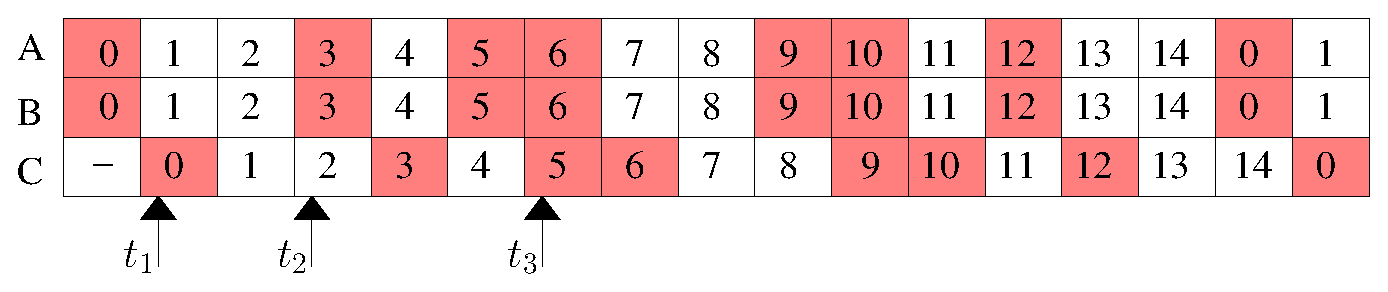
\includegraphics[width=.9\columnwidth]{figs/disco_example}
   \caption{Disco with a pair of primes (3, 5)} 
   \label{fig:disco_example}
\end{figure}

Probabilistic neighbor discovery protocols like Birthday~\citep{mcglynn2001birthday} 
have lower average-case discovery latencies, but the worst-case latency 
is unbounded. Deterministic protocols like Disco~\citep{Dutta2008Practical} 
and Searchlight~\citep{bakht2012searchlight} have slightly higher average 
discovery latencies but bounded worst-case latencies. Our key observation 
is that {\em slot index synchronization has a significant impact on the 
discovery latency for deterministic protocols}.

To illustrate this, Fig.~\ref{fig:disco_example} shows the discovery
process between three nodes that run Disco with the parameters (3, 5).
This gives a duty cycle of about 50\% and a period of 15 slots.  The
shaded and white boxes represent active and sleeping slots
respectively.  In this example, node A and B are strictly
synchronized, and node C is out-of-sync by one slot. Suppose all three
nodes come into contact at time $t_1$, node A and B will discover each
other at time $t_2$ with a latency of two slots, while node C will
discover the rest at time $t_3$ with a latency of five slots. It is
clear from this illustration that when the nodes are synchronized, the
worst-case latency is the largest gap between the active slots.

To investigate the improvement that can be achieved with synchronized
nodes, we enumerated all possible slot offsets between a pair of nodes
running the same symmetric protocol, and recorded the discovery
latency as the number of slots it takes from first contact to the
first intersecting active slot for the two nodes. We treated adjacent
active slots as a successful detection as well, because perfect
alignment rarely exists in real life and partially overlapping slots
are sufficient for detection. This is especially important for
BlindDate and Searchlight-S (Searchlight with striped probing) because
perfect alignment may cause failure of detection. To overcome this,
these protocols extend the active slot so as to ensure overlap of
adjacent active slots.


We computed the distribution of the discovery latency of the different
protocols with duty cycles of 5\% and
1\%~\citep{wang13blinddate, sun14hello, bakht2012searchlight}, and plot
the result for 5\% duty cycle in Fig.~\ref{fig:latency-cdf}. The
result for 1\% duty cycle is similar. Our analysis shows that, with
the same duty cycle, Searchlight-S is the best performing protocol
with the lowest average-case and worst-case latency.

\begin{figure}[t]
   \centering
   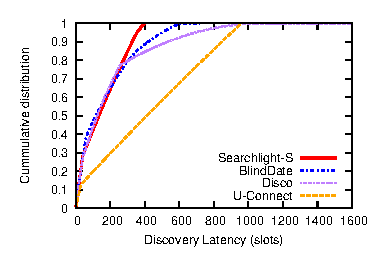
\includegraphics{graphs/analysis/latency-cdf}
   \caption{Cumulative distribution of discovery latency for the
		          various protocols at duty cycle of 5\%.}
   \label{fig:latency-cdf}
\end{figure}


\begin{table*}[t]\footnotesize
   \centering
   \caption{Average and worst-case discovery latency. Values in
		        brackets indicate the latency in seconds.}
     %\vspace{-6pt}
   \label{tab:latency}
   \begin{tabularx}{\textwidth}{@{}l *{7}{>{\centering\arraybackslash}X} @{}}
      \toprule
      & \multicolumn{2}{c}{{\em Overall Performance}} & \multicolumn{2}{c}{{\em Synchronized Index}} & \multirow{3}{\linewidth}[-2em]{\centering Average Latency Improvement} & \multirow{3}{\linewidth}[-2em]{\centering Worst-case Latency Improvement} & \multirow{3}{\linewidth}[-2em]{\centering Parameter(s)} \\
      \cmidrule[.5pt](r){2-3}
      \cmidrule[.5pt](l){4-5}
      Protocol & Average Latency & Worst-case Latency & Average Latency & Worst-case Latency  \\
      & (slots)[s]  & (slots)[s] & (slots)[s] & (slots)[s] \\
      \cmidrule(lr){2-2}
      \cmidrule(lr){3-3}
      \cmidrule(lr){4-4}
      \cmidrule(lr){5-5}
      & \multicolumn{7}{c}{\bf\scriptsize 5\% Duty-cycle, 25\,ms per slot} \\[-2pt]
      \cmidrule[.5pt](l){2-8}
      Searchlight-S   & 151 [3.78] & 399 [9.98] & 12.3 [0.31] & 37 [0.93] & 12.28 & 10.78 & 40\\
      BlindDate       & 168 [4.20] & 685 [17.13] & 13.8 [0.35] & 46 [1.15] & 12.17 & 14.89 & 12\\
      Disco           & 194 [4.85] & 1,071 [26.78] & 12.7 [0.32] & 36 [0.90] & 15.28 & 29.75 & (37, 43)\\
      U-Connect       & 423 [10.6] & 960 [24.00] & 14.6 [0.37] & 30 [0.75] & 28.97 & 32.00 & 31\\
									    
      & \multicolumn{7}{c}{\bf\scriptsize 1\% Duty-cycle, 5\,ms per slot} \\[-2pt]
      \cmidrule[.5pt](l){2-8}
      Searchlight-S   & 4,711 [23.56] & 9,999 [50.00]  & 65.7 [0.33] & 197 [0.99] & 71.70 & 50.76 & 200\\
      BlindDate       & 6,387 [31.94] & 17,821 [89.1]  & 71.4 [0.36] & 238 [1.19] & 89.45 & 74.88 & 60\\
      Disco           & 10,125 [50.6] & 35,655 [178] & 64.1 [0.32] & 180 [0.90] & 157.96  & 198.08  & (181, 211)\\
      U-Connect       & 11,123 [55.6] & 22,800 [114] & 74.6 [0.37] & 150 [0.75] & 149.10  & 152.00  & 151\\
      \bottomrule
  \end{tabularx}
\end{table*}

We also compared the average-case and worst-case latency of each
protocol against the case where both nodes have their slot indices
synchronized in Table~\ref{tab:latency}.  The key observation is that
the average and worst-case latency are significantly lower when the
nodes are synchronized on their slot indices. This result is intuitive
since two synchronized nodes follow the same sleep-wake pattern and
thus wake up at the same time.  What is surprising is the amount of
improvement. Even for the best performing protocol, Searchlight-S at
1\% duty cycle, the average latency is reduced by 72 times.  With the
slot size of 5\,ms, we can reduce the average latency from 24\,s to
0.33\,s, and the worst-case latency from 50\,s down to about 1\,s.

While slot index synchronization improves performance greatly, we
cannot always guarantee the synchronization between two nodes due to
the inherent errors in the sensor hardware. For example, the timing
signals are produced by electronic components, known as oscillators.
The oscillation frequency may vary due to different reasons such as
the temperature and vibration which is known as \emph{clock skew}.
Hence, the effectiveness of slot synchronization is dependent on the 
accuracy of synchronization.


\subsection{Distributed Synchronization Not Feasible}

In a docking application, static nodes are not able to communicate
with each other directly and have to rely on mobile nodes to relay
information. One approach to achieve synchronization would be to use a
distributed clock synchronization algorithm such as DCS~\citep{choi2012dcs}.  
The duty cycle of the nodes can then be derived from the resulting 
reference clock, and synchronizing their clocks will naturally 
synchronize the slot indices.

However, this approach does not work for two reasons. First, we have
found that DCS either fails or takes an extremely long time to
synchronize the clocks of nodes to within an accuracy of one slot
duration.  This means that either node indices will never be
synchronized, or the improvement would be small due to the long
convergence time.  Second, DCS is designed to work in a closed system,
where no nodes leave or join the system. Otherwise, it can no longer
guarantee convergence.  In our docking application, the mobile nodes
can leave and new mobile nodes may enter the system at any time.

Because of the shortcomings of the distributed algorithms, we adopt a
reference-based technique for synchronization, where a node is elected
to be the reference node that all other nodes synchronize with.  Our
key observation is that although the mobile nodes do not follow a
pre-determined path, the movement is not completely random.  Thus, we
exploited the movement pattern of tourists and designed a simple
algorithm to elect the reference node.

\section{Mobility-Assisted Slot Synchronization}
\label{sec:mass}

We have shown that slot index synchronization can significantly
improve latency. In this section, we describe the design of
Mobility-Assisted Slot index Synchronization (MASS) for our tourist
tracking application at Mogao Grottoes.

Since static nodes cannot directly communicate with each other, mobile
nodes are used to relay information between the static nodes.  The
challenge is that mobile nodes do not move along pre-determined
paths. Thus, we cannot determine prima facie which static node will be
visited next.  However, we observed from the traces of our real-world
application that the paths of the mobile nodes tend to follow a
certain set of patterns. We can exploit the patterns to elect
relatively stable reference nodes in a distributed manner, and have
the non-reference nodes synchronize their slot index with these
reference nodes. In addition, we use the clock of the reference node
as the reference clock for clock drift compensation.

All static and mobile nodes will adopt the same neighbor-discovery
protocol with a common set of parameters. Thus, if all (or most) of
the static nodes have their slot indices synchronized, mobile nodes
can likewise have their slot indices synchronized with every static
node. This results in a very small discovery latency when they come
into contact with any of the synchronized static nodes.

\subsection{Distributed Reference Election \& Synchronization}
\label{sec:selection}

\begin{figure}[t]
   \centering
   \begin{subfigure}
       \centering
       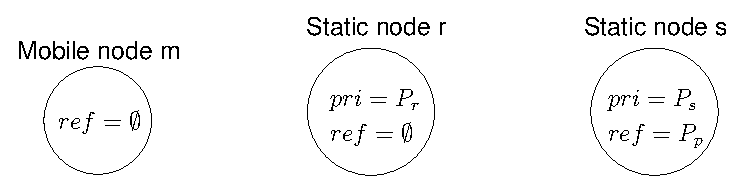
\includegraphics[scale=0.55]{figs/illustration-1}
   \end{subfigure}
      \parbox{.8\columnwidth}
      {\smallskip\scriptsize
      Mobile node $m$ has no initial reference. Static node $r$ also
      has no reference while static node $s$ has previously
      synced with node $p$.\\}
  \begin{subfigure}
      \centering
      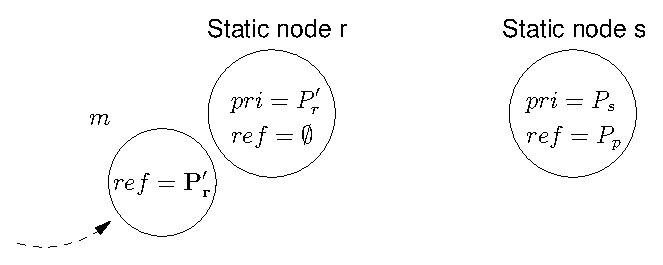
\includegraphics[scale=0.55]{figs/illustration-2}
  \end{subfigure}
      \parbox{.8\columnwidth}
      {\smallskip\scriptsize
      Node $m$ encounters node $r$, synchronizes with $r$ and
      updates its reference to $P_r$.\\}
  \begin{subfigure}
      \centering
      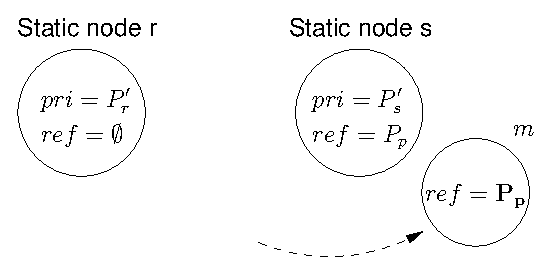
\includegraphics[scale=0.55]{figs/illustration-3}
  \end{subfigure}
      \parbox{.8\columnwidth}
      {\smallskip\scriptsize
      Now $m$ leaves and encounters node $s$. Suppose $P_r'<P_s'$
      and $P_s'<P_p$, node $m$ syncs with node $s$ and updates its
      reference to $P_p$.\\}
  \begin{subfigure}
      \centering
      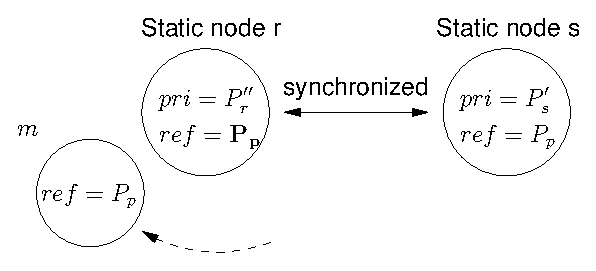
\includegraphics[scale=0.55]{figs/illustration-4}
  \end{subfigure}
      \parbox{.8\columnwidth}
      {\smallskip\scriptsize
      Suppose now $m$ returns to node $r$, and suppose even after
      updating $P_r''$, $P_r''<P_p$, then node $r$ will sync with $m$
      and record $P_p$ as its reference. Now nodes $r$ and $s$ will be
      in sync.\\}
  \caption{Reference node election.} 
  \label{fig:selection}
\end{figure}

\begin{table}[t]\scriptsize
   \centering
   \caption{Summary of update rules for reference node election}
      %\vspace{-6pt}
   \begin{tabularx}{\columnwidth}{@{}lll@{}}
     \toprule
     Condition & Static node & Mobile node \\
     \midrule
       $P_{m} > max(P_{s}, P_{s.ref})$ & $P_{s.ref} \leftarrow P_m$ & No Change \\
       $P_{m}<max(P_{s}, P_{s.ref})$ & No Change & $P_m \leftarrow \textrm{max}(P_s, P_{s.ref})$ \\
     \bottomrule
   \end{tabularx}
   \label{tab:priority}
\end{table}

To elect the reference nodes, we introduce the notion of a priority
metric $P$.  Each static node $s$ computes a priority $P_s$ based on
information carried by the mobile nodes in a distributed way. In
addition, each static node $s$ also stores the recorded priority of
its reference, $P_{s.ref}$ obtained from the mobile nodes. Similarly,
each mobile node, $m$, also stores the priority ($P_m$) of the last
static node that it is synchronized with. When a mobile node $m$
encounters a new static node $s$, the static node first updates its
priority $P_s$. Then, the priorities $P_s$, $P_{s.ref}$, and $P_m$ are
compared and exchanged.

If $P_m$ is larger than $P_s$ and $P_{s.ref}$, then the static node
will synchronize its clock and slot index according to that of the
mobile node, and set its reference $P_{s.ref}$ to $P_m$. Indirectly,
the static node will have now synchronized with the static node that
the mobile node has last synchronized with. On the other hand, if
$P_m$ is smaller than $P_s$ or $P_{s.ref}$, the mobile node will
synchronize its slot index with the static node.  It will also
set its reference $P_m$ to the larger of $P_s$ and $P_{s.ref}$.
Fig.~\ref{fig:selection} illustrates the steps of this process and
Table~\ref{tab:priority} summarizes the above update rules. With this
simple algorithm, the node with the largest priority value will be
elected as the reference node, from which other nodes will take
reference.  It remains for us to describe how a static node $s$
determines and computes its priority $P_s$.

\begin{figure}[t]
   \centering
   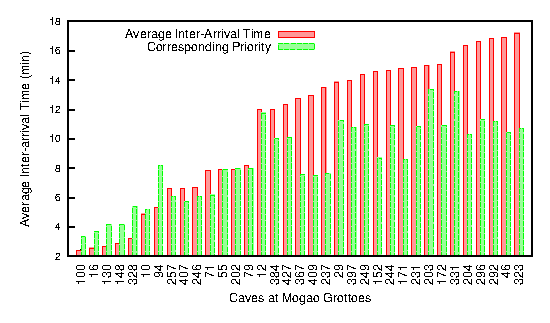
\includegraphics[scale=0.85]{graphs/visiting_frequency/visitingfrequency}
   \caption{Average inter-arrival time and the priority of different
            caves at Mogao Grottoes over one day.}
   \label{fig:visitingfrequency}
\end{figure}

{\bf Node Priority}. For our reference node election algorithm to work
well, not only does the priority $P_s$ need to be a metric that can be
easily computed in a distributed way, the resulting priority for
different static nodes should also preferably be distinct. In our
docking application, we observed that some caves were more popular
than others due to either its intrinsic attractiveness to the
tourists, or its relative location, i.e., it might be near route
entrances. Such caves will have more visitors than others. Thus, we
decided to utilize the average inter-arrival time between mobile nodes
at each static node $s$ to obtain its priority $P_s$.

The static nodes compute $P$ by measuring the time elapsed since the
last visit to the cave. The priority is accumulated using an
exponentially-weighted moving average (EWMA) with a smoothing factor
$\alpha = \frac{1}{8}$.  In other words, the equation to update $P_i$
to $P_{i+1}$ is:
\begin{equation}\label{eq1}
	P_{i+1} = \alpha t + (1 - \alpha) P_i
\end{equation}
where $t$ is the elapsed time since the last visit to this cave.

In Fig.~\ref{fig:visitingfrequency}, we plot the actual average
inter-arrival time of each cave over one day of a real trace and the
computed priority $P_i$.  Although the computed priority is often not
close to the actual daily average values, the trends are similar,
i.e., the more frequently visited nodes will have a higher priority.

It is entirely plausible that for some docking applications, the
static nodes have similar visiting frequencies and the computed
priorities might be very close to one another. In such cases, the
inter-arrival time might not be the best metric and another metric
could be used. However, our reference election algorithm is still
applicable if a good metric can be found.

\subsection{Clock Drift Compensation \& Slot Synchronization}
\label{sec:clock-drift}

\begin{figure*}[t]
   \centering
   \subfigure[Mean and variance of clock skew measured at one node using different
   time intervals]{
       \centering
       \begin{minipage}[t]{0.32\textwidth}
          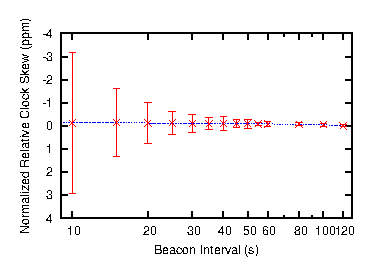
\includegraphics[scale=0.85]{graphs/clock_skew_measure/skew_interval}
          %\caption{Mean and variance of clock skew measured at one node using different
	      %time intervals.}
          \label{fig:skew_int}
       \end{minipage}}
   \subfigure[Clock skew measured at 1-min intervals between the sending node and
   receiving nodes]{
       \begin{minipage}[t]{0.32\textwidth}
          \centering
          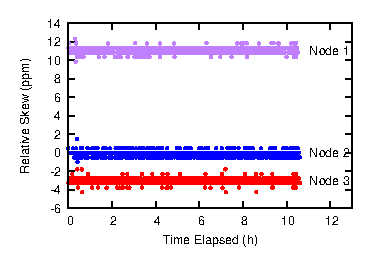
\includegraphics[scale=0.85]{graphs/clock_skew_measure/fournodes_skew_1minute}
          %\caption{Clock skew measured at 1-min intervals between the sending node
         %receiving nodes.}
          \label{fig:skew_minute}
       \end{minipage}}
   \subfigure[Amount of clock drift between two ndoes with and without clock drift compensation]{
       \begin{minipage}[t]{0.32\textwidth}
          \centering
          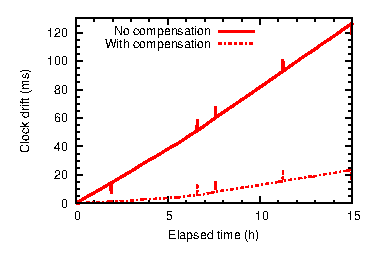
\includegraphics[scale=0.85]{graphs/clock-drift-experiment/cdc}
          %\caption{Amount of clock drift between two nodes with and without clock drift compensation.}
          \label{fig:skew_cdc}
       \end{minipage}}
   \caption{Clock skew of the three receiving nodes.}
   \label{fig:skew}
\end{figure*}


Once a reference node is elected, each node will synchronize their
clocks to that reference node. However, clock drift will introduce
errors, even if a node is perfectly synchronized at the start.  Hence,
both static and mobile nodes in our system must continuously estimate
and compensate for clock drift.

{\bf Clock Skew Estimation.}  There are many existing algorithms for
clock skew detection and
estimation~\citep{hamilton2008aces,yang2010adaptive,liao2013distributed}.
Zhong et al.\ showed that it is possible to continuously detect and
estimate the clock skew between two nodes~\citep{zhong2011demand}.  We
believe that any of the state-of-the-art techniques could be used for
MASS. For validation, we performed a simple experiment: a sensor node
periodically sends beacons at different intervals to three sensor
nodes that keep listening to compute relative clock skew, using the
following formula~\citep{huang2013psr, xu2013taco}:
\[
	\delta_{AB} = \frac{(t^A_{i+1} - t^A_i) - (t^B_{i+1} - t^B_i)}
	{t^A_{i+1} - t^A_i}
\]
where $t^A_i$ and $t^B_i$ are the local time at the sender's and
receiver's clock when the $i$th beacon was sent and received. The
MAC-layer time-stamping technique was used to mitigate the variance of
the delivery time~\citep{maroti2004flooding}.

In Fig.~\ref{fig:skew_int}, we plot the average estimated relative
clock skew and the standard deviation in parts per million (ppm) for
beacon intervals from 1\,s to 120\,s based on the sensor nodes used
in the tracking system at Mogao Grottoes which will be introduced in 
Section~\ref{sec:mock-up}. We found that a larger beacon
interval leads to a more accurate and stable estimation.  In
Fig.~\ref{fig:skew_minute}, we plot the relative clock skew between
the sending node and the three receiving nodes with the beacon
interval of 60\,s over a few hours.  We observed that the three
receiving nodes can reliably detect and measure their relative clock
skew against the sending node with an error within 1.5\,ppm. In
Fig.~\ref{fig:skew_cdc}, we plot the time difference between the
clocks of two nodes with and without clock drift compensation, which
suggests that it is possible to estimate and compensate for the clock
drift in our system.

From the real Mogao Grottoes traces, tourists (and therefore the mobile
nodes) will typically stay in each cave for more than 120\,s
(see~Fig.\ref{fig:cdf_duration}), which as Fig.~\ref{fig:skew_int}
suggests, is sufficiently long to get a good estimate of the clock
skew. Since the average inter-arrival time of the mobile nodes at each
cave is less than 18 minutes (see Fig.~\ref{fig:visitingfrequency}),
the expected clock drift during this interval is within one slot
(5\,ms) with clock drift compensation.

\begin{figure}[t]
   \centering
   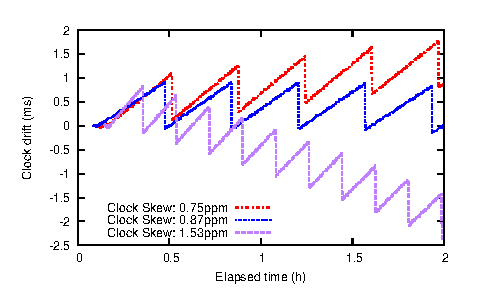
\includegraphics{graphs/clock-compensation-result/compensate-effect}
   \caption{Clock drift changes with dynamic compensation interval for three mobile nodes.}
   \label{fig:compensation}
\end{figure}

{\bf Clock Drift Compensation.} Once we have an estimate of the clock
skew, sensor nodes can compensate for its clock drift against the
reference node by adjusting its clock periodically. Due to the
granularity of the clocks~(30~$\mu s$ for our hardware), the compensation
interval cannot be too small. We found that having the nodes adjust 
their clocks every 100\,s worked well for our sensor hardware as shown 
in Fig.~\ref{fig:skew_cdc} where the clock drift between two nodes can
be reduced by 8 times compared with no compensation.

However, in practice, it is difficult to set an appropriate compensation
interval since the relative clock skew between nodes is not known in advance.
Thus, instead of using a constant compensation interval, we set an clock
drift tolerance to make each node automatically compute the compensation
interval which we call the dynamic compensation interval. Through the 
measurement on our hardware, it is effective to set the clock drift tolerance 
1~ms.

We validate such dynamic compensation interval with the neighbor discovery
protocol. We choose four nodes where one node works as the static node while 
the other three as the mobile nodes. These four nodes run the Searchlight 
protocol with 5\% duty cycle and 5~ms slot size. Mobile nodes do slot index 
synchronization with the static node after the first discovery. After 120~s, 
the three mobile nodes estimate the relative clock skew with the static node. 
Then each mobile node compute its compensation interval and do clock drift
after the interval.

We compute the wake up time drift after each discovery period and plot the
results in Fig.~\ref{fig:compensation}. We can see that in the compensation 
interval the clock drift becomes larger and will be revised with compensation. 
Ideally, with periodic compensation, the mobile nodes can keep slot index 
synchronization with the static node. However, it is difficult to achieve 
perfect slot index synchronization in practice due to measurement errors 
including clock skew estimation error, compensation error and the dynamic 
varrations of oscillator frequency. However, with our proposed clock drift 
compensation method, the slot index synchronization can be extended to 2.3~hours, 
5.25~hours and 6.15~hours compared to the initial 0.77~hour, 1.15~hours and 
1.75~hours without compensation for the three mobiles respectively.

{\bf Slot Alignment} While it is possible for the nodes to align their
slot timing to the reference node, we found that the resulting
improvements from doing so are marginal. As such, we adopt a simple
index synchronization process --- the nodes simply update the current
slot index to the reference node's slot index. Because every node is
running the same neighbor discovery protocol, every active slot of
such synchronized pairs of nodes will overlap.

\subsection{Mitigating the Pitfalls of Small Synchronization Errors}
\label{subsec:pitfall}

\begin{figure}[t]\footnotesize
   \hfill
   \subfigure[SL-S]{
        \centering
	\begin{minipage}[b]{0.3\columnwidth}
           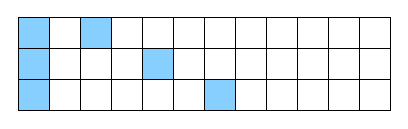
\includegraphics[width=1\textwidth]{figs/searchlight}
	   \label{fig:searchlight}
	\end{minipage}}
   \hfill
   \subfigure[SL-S+1]{
        \centering
	\begin{minipage}[b]{0.3\columnwidth}
	   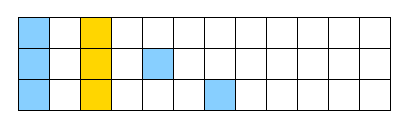
\includegraphics[width=1\textwidth]{figs/searchlight+1}
	   \label{fig:searchlight+1}
        \end{minipage}}
   \hfill
   \subfigure[SL-S+1/2]{
        \centering
	\begin{minipage}[b]{0.3\columnwidth}
           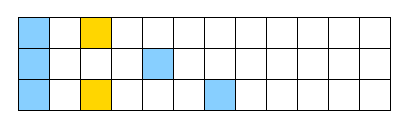
\includegraphics[width=1\textwidth]{figs/searchlight-1}
           \label{fig:searchlight+1/2}
	\end{minipage}}
   \hfill
   \caption{Additional active slots to the Searchlight-S protocol with
      $p=12$.}
   \label{fig:searchlights}
\end{figure}

Even with clock drift compensation, we cannot guarantee perfect
synchronization all the time. It turns out to be a big problem that
can potentially lead to the worst-case scenario for discovery latency.
In particular, an offset of two slots will result in the
worst-case scenario for Searchlight-S (the optimal symmetric
protocol)~\citep{sun14hello}.

To overcome this potential pitfall, we introduce a small modification
to the duty-cycle pattern for the neighbor discovery protocol by
adding an extra number of active slots. We illustrate this with
Searchlight-S.  In Searchlight-S, nodes wake up at every $p$ slots and
a probe slot traverses from the first position to $p/2$ across $p/2$
sub-cycles (see Fig.~\ref{fig:searchlight}), resulting in a period
of $p(p/2)$. To prevent the worst-case latency from occurring when the
cycles of two nodes have an offset of 2, we set the node to wake up at
every $kp+2$ slots (see Fig.~\ref{fig:searchlight+1}). We call this
scheme {\em Searchlight+1}. With the additional active slots, the duty
cycle of Searchlight+1 will be $1.5$ times that of Searchlight with
the same $p$. To keep the duty-cycle constant, $p$ has to be increased
by $1.5$ times, thereby incurring a slightly larger latency. One
possible way to reduce this additional delay is to halve the number of
extra active slots by only introducing them every 2 sub-cycles (See
Fig.~\ref{fig:searchlight+1/2}). We call this modified scheme {\em Searchlight+1/2}.

\begin{table}[t]\footnotesize
   \centering
   \caption{Combined latencies of the modified Searchlight protocols
       for cycles offset by 0 and 1 at 5\% duty-cycle.}
   %\vspace{-6pt}
   \begin{tabularx}{\columnwidth}{@{}l *{6}{>{\centering\arraybackslash}X}@{}}
      \toprule
      & \multicolumn{2}{c}{SL-S} & \multicolumn{2}{c}{SL-S+1} & \multicolumn{2}{c}{SL-S+1/2} \\
      \cmidrule(lr){2-3}
      \cmidrule(lr){4-5}
      \cmidrule(lr){6-7}
      & \multicolumn{6}{c}{Latency (slots)} \\
      & Avg & Worst & Avg & Worst & Avg & Worst \\
      \cmidrule(lr){2-2}
      \cmidrule(lr){3-3}
      \cmidrule(lr){4-4}
      \cmidrule(lr){5-5}
      \cmidrule(lr){6-6}
      \cmidrule(lr){7-7}
      Offset 0, 1 &  12.3 & 37  & 18.5 & 57  & 15.3 & 47 \\ 
      Offset 2    & 199.5 & 399 & 29.4 & 59  & 47.6 & 99 \\
      Offset 3    & 163.5 & 359 & 29.2 & 59  & 43.4 & 99 \\
      \cline{2-7}
      Average     & 125.1 & 265 & 25.7 & 58.3 & 35.4 & 81.7 \\ 
      \bottomrule
   \end{tabularx}
   \label{tab:latency-aligned}
\end{table}

We compared the average-case and worst-case latencies for our
modifications when the slots indices are offset by 0, 1, 2 and 3, to
Searchlight-S in Table~\ref{tab:latency-aligned}.  We see that the
latencies when the slots are offset by 2 can be significantly reduced,
at the cost of slightly longer cycles, which increases the overall
latency by a small amount. Fig.~\ref{fig:searchlight-cdf} shows that
our modified schemes slightly increase the overall latency.

\begin{figure}[t]
   \centering
   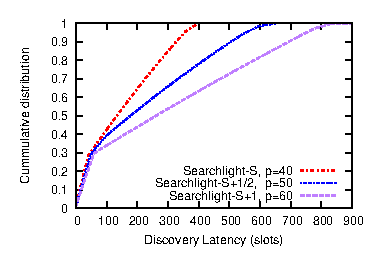
\includegraphics{graphs/analysis/searchlight-cdf}
   \caption{Distribution of latency for the modified Searchlight
          protocols at 5\% duty cycle.}
   \label{fig:searchlight-cdf}
\end{figure}


\section{Evaluation}
\label{sec:eval}

In this section, we evaluated the effectiveness of MASS in enhancing
existing deterministic neighbor discovery protocols using our custom
trace-based simulator.  Our simulator simulates the interactions
between the mobile and static nodes using the real traces of tourist
movements collected at Mogao Grottoes.  The operating hours of the
Mogao Grottoes are from 8:00\,am to 6:00\,pm daily, so we have
approximately 10 hours of data for each day.  The data set used for
our simulations consists of 31 days of traces over the one-month
period in August 2013, containing 8,658 movement routes for the mobile
nodes and 69,271 cave visits.  As an example, the routes for a
particular day are shown in Fig.~\ref{fig:trace}, where each cave is
assigned a unique ID.

\begin{figure}[t]
    \centering
    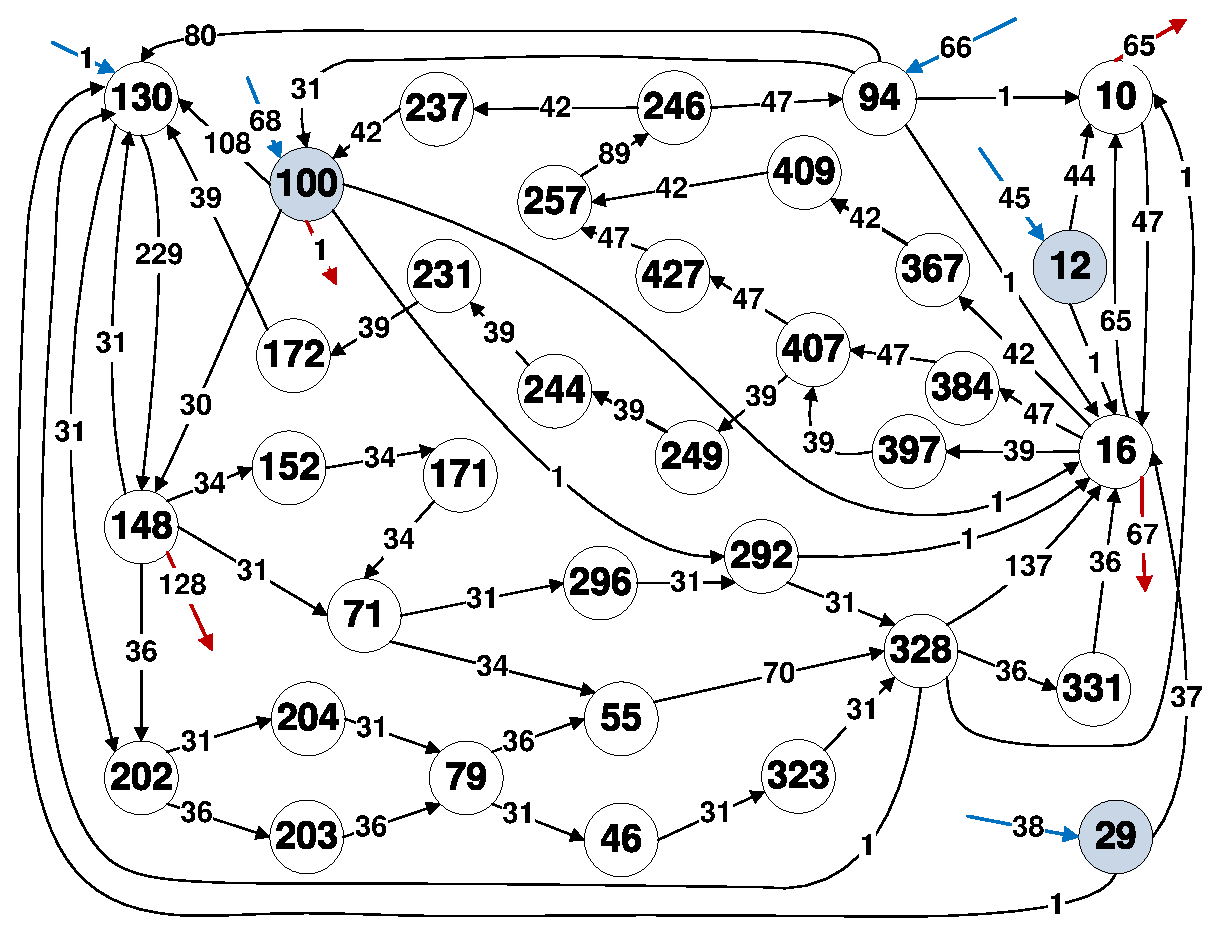
\includegraphics[scale=0.30]{static/path1}
    \caption{Visiting route of the tour groups at Mogao Grottoes on 1
             Aug 2013.  The number on the arrows indicates the number of mobile
             nodes that took that path.  Shaded caves indicate the reference
             nodes elected by the end of the day.}
    \label{fig:trace}
\end{figure}

\subsection{Power Conservation and Latency Reduction}

\begin{figure*}[t]
    \centering
    \subfigure[5\% duty cycle and 25\,ms slot size.]{
        \begin{minipage}[b]{0.33\textwidth}
          \centering
          %\includegraphics{graphs/A_C_together_break-25ms-5/a_c_break-25ms-5-orig}
	  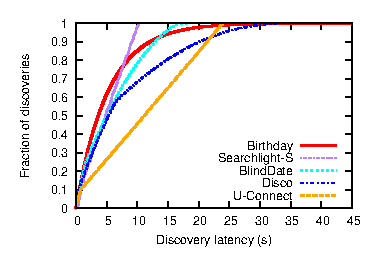
\includegraphics[scale=0.85]{graphs/one-month-result/august-25ms-5-orig}
          %\caption{5\% duty cycle and 25\,ms slot size.}
          \label{fig:a_c_break-25ms-5-orig}
	\end{minipage}}%
    \subfigure[1\% duty cycle and 25\,ms slot size.]{
        \begin{minipage}[b]{0.33\textwidth}
          \centering
          %\includegraphics{graphs/A_C_together_break-25ms-1/a_c_break-25ms-1-orig}
	  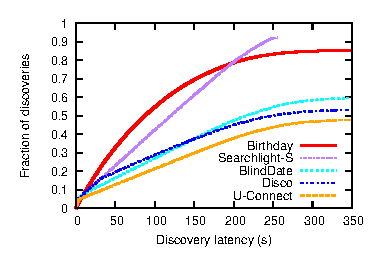
\includegraphics[scale=0.85]{graphs/one-month-result/august-25ms-1-orig}
	  %\caption{1\% duty cycle and 25\,ms slot size.}
	  \label{fig:a_c_break-25ms-1-orig} 
	\end{minipage}}%
    \subfigure[Duration of mobile nodes stay in caves]{
        \begin{minipage}[b]{0.33\textwidth}
          \centering
          %\includegraphics{graphs/duration_cdf/cdf_together_duration}
	  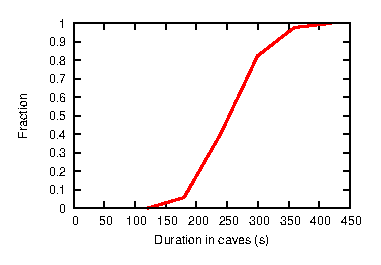
\includegraphics[scale=0.85]{graphs/one-month-result/cdf_august_duration}
          %\caption{Duration of mobile nodes stay in caves} 
          \label{fig:cdf_duration}
	\end{minipage}}
    \caption{Impact of reducing duty cycle from 5\% to 1\% for
       Birthday, BlindDate, Disco, Searchlight and U-Connect.}
    \label{fig:break-orig}
\end{figure*}

\begin{figure*}[t]
    \centering
    \subfigure[No synchronization]{
        \begin{minipage}[b]{0.33\textwidth}
           \centering
           %\includegraphics{graphs/A_C_together_break-5ms-1/a_c_break-5ms-1-orig}
	   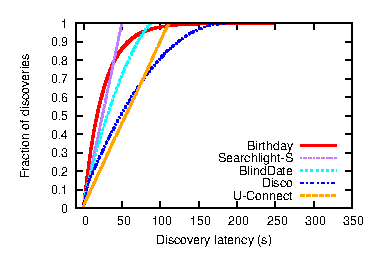
\includegraphics[scale=0.85]{graphs/one-month-result/august-5ms-1-orig}
           %\caption{No synchronization.}
           \label{fig:a_c_break-5ms-1-orig}
        \end{minipage}}%
    \subfigure[With DCS]{
        \begin{minipage}[b]{0.33\textwidth}
           \centering
           %\includegraphics{graphs/A_C_together_break-5ms-1/a_c_break-5ms-1-dcs}
           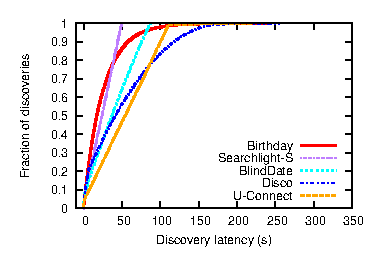
\includegraphics[scale=0.85]{graphs/one-month-result/august-5ms-1-dcs}
           %\caption{With DCS.}
           \label{fig:a_c_break-5ms-1-dcs} 
        \end{minipage}}%
    \subfigure[With MASS]{
        \begin{minipage}[b]{0.33\textwidth}
           \centering
           %\includegraphics{graphs/A_C_together_break-5ms-1/a_c_break-5ms-1-syn}
           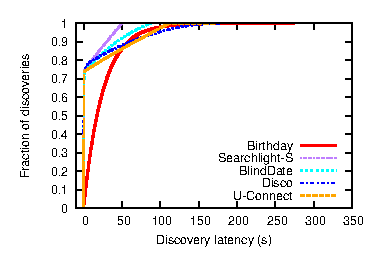
\includegraphics[scale=0.85]{graphs/one-month-result/august-5ms-1-syn}
           %\caption{With MASS.}
           \label{fig:a_c_break-5ms-1-syn}
        \end{minipage}}
    \caption{Discovery latency of each protocols and MASS and DCS
        assisted versions at 1\% duty cycle and 5\,ms slot size.}
    \label{fig:break-compare}
\end{figure*}


In neighbor discovery protocols, the power saving is determined by the
duty cycle, which is the proportion of time that a node stays
active. The typical duty cycles used in these protocols are 1\% and
5\%, and the slot size is typically
25\,ms~\citep{wang13blinddate,sun14hello,bakht2012searchlight}.

In Fig.~\ref{fig:a_c_break-25ms-5-orig}, we plot the cumulative
distribution of the discovery latency of the five most common neighbor
discovery protocols using a 5\% duty cycle and a slot size of
25\,ms. We see that as expected, Searchlight-S is the best
deterministic protocol, which is consistent with our earlier analysis.

As energy consumption is an important factor in docking applications,
we tried to reduce energy consumption by decreasing the duty cycle to
1\% (while maintaining the original slot size of 25\,ms) and plot the
results in Fig.~\ref{fig:a_c_break-25ms-1-orig}.  The discovery
latency for all protocols increased by about a factor of
10. Furthermore, the worst-case latency can now be longer than the
time that the tourists spend in the caves, which can potentially cause
detection failures. We plot the distribution of the time that the
mobile nodes spend in the caves in Fig.~\ref{fig:cdf_duration},
which confirms our intuition and shows that the worst-case neighbor
discovery latency needs to be below 200\,s for the reliable tracking
of tourists.

We can reduce the discovery latency by using a smaller slot size.
However, how small we can go depends on the hardware and operating
system of the nodes.  Zhang et al.\ suggested that the smallest
feasible size for a slot is 5\,ms, because any smaller size will cause
jitter and make the system unstable~\citep{zhang2012acc}. Also, 5\,ms
of air time might be insufficient to exchange usable data. However, we
argue that once discovery happens, the nodes can switch to a different
communication protocol for the exchange of information.  Thus, we set
the slot size to 5\,ms with a duty cycle of 1\% and plot the new
cumulative distribution of the discovery latency in
Fig.~\ref{fig:a_c_break-5ms-1-orig}. We see that as expected, the
discovery latency improves, but the latency increases to almost 5
times that of the original as in Fig.~\ref{fig:a_c_break-25ms-5-orig}.

{\bf Adding Synchronization}. Next, we investigated how
synchronization would improve discovery latency. We repeated the
simulation with a duty cycle of 1\% and a slot size of 5\,ms after
introducing synchronization with DCS and MASS. We plot the results in
Fig.~\ref{fig:a_c_break-5ms-1-dcs}
and~\ref{fig:a_c_break-5ms-1-syn} respectively.

As expected, synchronization has no impact on the performance of the
Birthday protocol. Although in general, synchronization improves the
latency for deterministic protocols, the improvements with DCS are
marginal. This is because DCS is not able to converge sufficiently
fast in our scenario. For MASS, the discovery latency for the same
protocols was reduced to less than one second about 75\% of the time,
which suggests that most of the nodes were successfully synchronized. 
However, even with MASS, the worst-case latency remained the same.
The reason is either some nodes could not be synchronized or they had 
to be re-synchronized at the start of each day. For example, the cave
12 and cave 29 at Mogao grottoes are usually the first cave visited
which means that the mobile nodes can not relay synchronization 
information to them. Thus, the static nodes in these two caves can
not synchronize with the selected reference node.

The reduction in discovery latency is important for our tourist
tracking application because our goal is to learn the relationship
between the number of tourists and the changes of micro-climate such
as the tempperature, humidiy and carbon dioxide in the caves. It is
essential to accurately track the duration of stay for tourists in 
each cave. The median time that visitors spend in each cave is 250\,s. 
Detecting the visitors with a 25\,s delay (at 1\% duty cycle) results 
in an error of 10\%. By reducing the discovery latency to less than 
1\,s, we can improve the estimation accuracy by more than 20 times.

\subsection{Performance gains using MASS}

\begin{figure}[t]
   \centering
   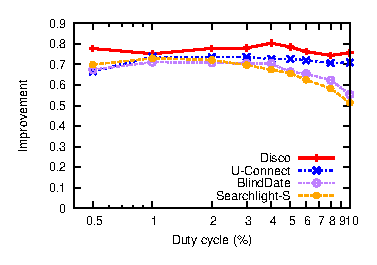
\includegraphics{graphs/protocols_improvement/improve}
   \caption{Improvement for various protocols with MASS
      under different duty cycles with 5\,ms slot size.}
   \label{fig:improve}
\end{figure}


\begin{figure*}[t]
   \minipage[t]{0.3\textwidth}
   \centering
   \vspace{0pt}
   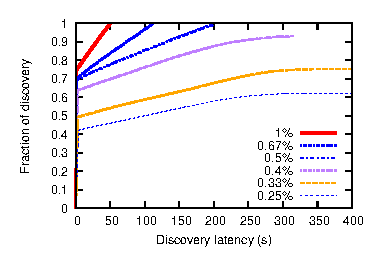
\includegraphics[scale=0.85]{graphs/one-month-result/august-low-syn}
   \caption{Distribution of discovery latency of Searchlight-S with
      MASS at very low duty cycles.}
   \label{fig:small}
   \endminipage\hfill
   \minipage[t]{0.33\textwidth}
   \centering
   \vspace{0pt} 
   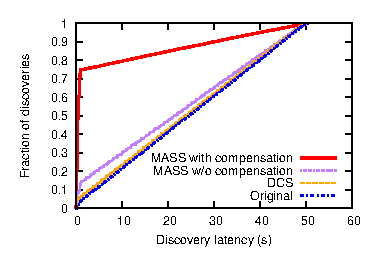
\includegraphics[scale=0.85]{graphs/one-month-result/august-5ms-1-anc-searchlight-strip}
   \caption{Distribution of discovery latency for Searchlight-S
        without clock drift compensation under 1\% duty cycle and 5\,ms
        slot size.}
   \label{fig:a_nc_break-5ms-1-searchlight}
   \endminipage\hfill
   \minipage[t]{0.3\textwidth}
   \centering
   \vspace{0pt} % anchor for minipage to align
   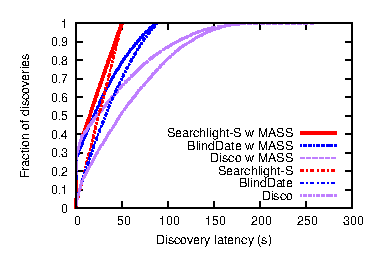
\includegraphics[scale=0.85]{graphs/one-month-result/august-random-5ms-1}
   \caption{Distribution of discovery latency with random routes.} 
   \label{fig:a_c_random-5ms-1}
   \endminipage\hfill
\end{figure*}


As the duty cycle affects the discovery latency of neighbor discovery
protocols, we plot the percentage improvement of the average discovery
latency with MASS over the original protocols in
Fig.~\ref{fig:improve}. An improvement of 90\% means that the
resulting average discovery latency with MASS is 10\% of the original
latency. The results show that as the duty cycle increases, the
improvement decreases for Searchlight-S and BlindDate.  This is
because at larger duty cycles, the original protocols already achieved
relative low discovery latencies and there is little room for
improvement. On the other hand, Disco and U-Connect show the same
improvement across different duty cycles.

Reducing duty cycles is beneficial to save power, but at a cost of the
increased discovery latency.  We examined how MASS affects this trade
off by further reducing the duty cycle while keeping the slot size at
5\,ms. Fig.~\ref{fig:small} shows the distribution of the discovery
latency for Searchlight-S with MASS using smaller duty cycles. Because
Searchlight-S has the lowest worst-case latency, we could reduce the
duty cycle to 0.5\% while maintaining 100\% discovery success rate in
our application. As expected, MASS still manages to keep the discovery
latency extremely low 75\% of the time. That is, decreasing the duty
cycle does not affect the improvements of MASS.  Only the worst-case
latency is affected.

\subsection{Effectiveness of Clock Skew Compensation}

Typical clock skew ranges from $\pm5$~ppm to
$\pm100$~ppm~\citep{zhong2011demand}.  We showed experimentally that it
is possible for clocks to drift apart by 5\,ms in just one hour (See
Fig.~\ref{fig:skew_cdc}). If the relative clock skew is 20\,ppm, and
since the average inter-arrival time of the mobile nodes in our
application is 15 minutes (See Fig.~\ref{fig:visitingfrequency}),
their clocks would have drifted apart by 18\,ms, which is much larger
than our slot size of 5\,ms. This would suggest that clock drift
compensation is essential to ensure the synchronization among the
nodes.

To validate this intuition, we repeated our experiments without clock
drift compensation and compared MASS and DCS using the Searchlight-S
protocol in Fig.~\ref{fig:a_nc_break-5ms-1-searchlight}.  As
expected, DCS has no impact on Searchlight-S. Without clock drift
compensation, the improvement of MASS is very limited. The same trends
are observed for the other neighbor discovery protocols.  This
demonstrates that clock drift compensation is essential to maintain
the synchronicity among the nodes.


\subsection{Random Traces}

Our MASS algorithm exploits the natural visiting patterns of the
mobile nodes in a docking application for synchronization.  In this
section, we examine how MASS performs if the visiting patterns are
completely random. To ensure a fair comparison, we generated random
traces that had the same node distribution as our Mogao Grottoes
traces.

Fig.~\ref{fig:a_c_random-5ms-1} shows the distribution of the
discovery latencies for Disco, BlindDate and Searchlight-S with and
without MASS. The results show that while MASS could still improve the
latency 30\% of the time, it is not as effective as before (75\% of
the time).  This is because we used the inter-arrival time as the
metric for MASS, which is random in the generated traces. Thus, our
reference election algorithm could not maintain a fixed reference node
for a prolonged period of time. This highlights that the selection of
the metric is a key factor that affects the overall performance for
MASS in docking applications.

\section{Experiments in a Mock-up Scenario}
\label{sec:mock-up}
We have shown that the discovery latency of existing neighbor discovery
protocols can be greatly improved with MASS. However, it is not clear 
how MASS will perform on a real sensor network. It is difficult and
unrealistic to thoroughly investigate its performance at Mogao Grottoes
since the current tourists tracking system is running and a sudden break
is not allowed. Thus, we mock up a similar scenario to evaluate the 
performance of the proposed MASS. We now describe our implementation and
practical considerations in the mock-up scenario.

\subsection{Hardware Platform}
\begin{figure}[t]
   \centering
   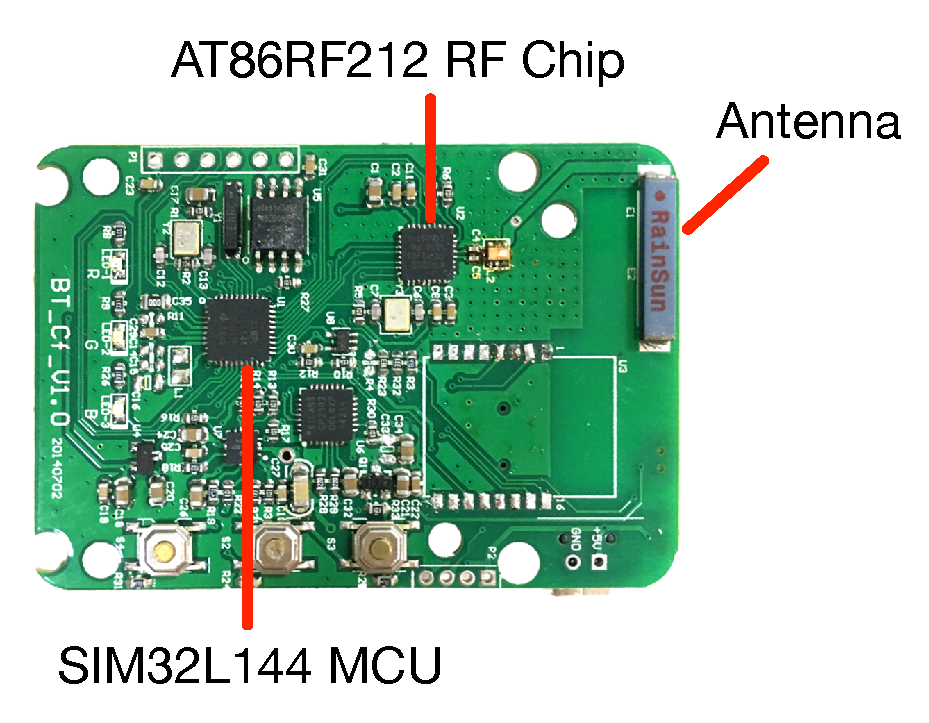
\includegraphics[width=.7\columnwidth]{static/sensor}
   \caption{Custom sensor platform}
   \label{fig:node}
\end{figure}

We use the same hardware platform in experiments as the nodes deployed
at Mogao Grottoes (shown in Fig.~\ref{fig:node}). The sensor node 
consists of a 32-bit ARM Cortex-M3 MCU SiM3L144 with 64~KB in-system
self-programmable flash and a low-power IEEE-compatible radio transceiver 
AT86RF212 operating at 700/800/900 MHz with the transmission rate from 
20 to 250~kbps. An important feature of sensor nodes is the low power 
property, with the working and sleeping current 30 mA and 1.2 $\mu$A 
respectively. A rechargeable 3.7V Li-Polymer battery is used to power 
the sensor node. The sensor nodes do not run any sensor operating systems
and are programmed directly in C. This is an advantage for our evaluation 
since it has been shown that sensor operating systems such as TinyOS often
introduce additional jitters~\citep{zhang2012acc} when the slot size is small.

\subsection{Mock-up Scenario and Setup}
\begin{figure}[t]
   \centering
   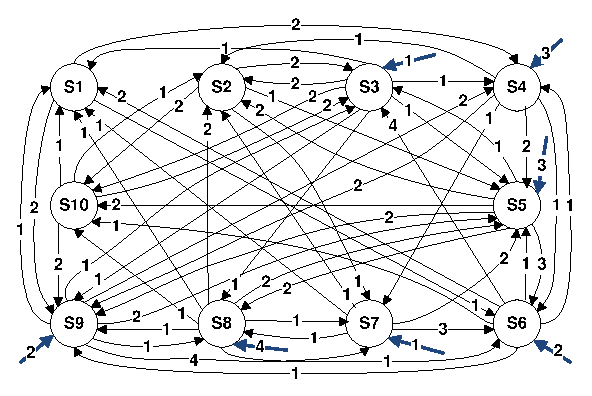
\includegraphics[width=.9\columnwidth]{static/route-1}
   \caption{Moving traces of 16 volunteers in the mock-up scenario over one day}
   \label{fig:mockup}
\end{figure}

{\bf Mock-up Scenario}. The mock-up scenario is designed on the third floor of a
building. Ten rooms are selected and in each room we deployed a static node. To 
simulate the radio signal blocking phenomenon between the caves at Mogao Grottoes, 
the signal transmitting power of static sensor nodes is reduced so that the mobile 
node can hear the beacons only when it enters the room. Then we invite volunteers 
to move through rooms with mobile nodes based on the predefined traces. The traces 
are randomly produced based on the statistics of the real trace in one month at 
Mogao Grottoes including the visiting sequence and the staying time distribution in 
each cave. Fig.~\ref{fig:mockup} shows the produced moving trace over one day. The 
numbe on the arrows indicates the number of volunteers moving and the shaded cave 
indicate the reference nodes elected by the end of the day.

{\bf Heterogeneous Working Pattern}. Existing neighbor discovery protocols generally 
adopt a beacon-listen-beacon working pattern in active slots. This arrangement seems 
logical since it enables a pair of nodes to hear each other's beacon and achieve 
mutual discovery when their active slots overlap. However, such working pattern is
not the optimal in our tracking application. It has been shown that when the slot
is aligned there will be beaconing collision when the active slots overlap which will
increase the discovery latency. To avoid beaconing collision with MASS, we adopt 
heterogeneous working patter for the static node and mobile node, i.e., the static 
node adopt the typical beacon-listen-beacon pattern while the mobile node firstly keeps 
listening in active slots and sends beacons if it receives the beacons from static nodes.
In this case, the discovery will happen once the active slots of two neighbors overlap.

{\bf Experimental Setup}. We adopted the state-of-the-art Searchlight-S with 1\% duty 
cycle and 5~ms slot size. Each beacon contains a 24-byte payload which includes 
necessary information for discovery such as the node ID, slot index, time counters and
priority changes. The total length of the underlying physical message is 41 bytes (4~B 
of preamble + 1~B of SFD + 1~B of PHR + 9~B of MHR + 24~B of MAC payload + 2~B of FCS).
With the data rage of 250~kbit/s, it will take nearly 1.5~ms to transmit one beacon.
The experiments last for three days and there are totally 271 discovery records with 
32 volunteers invited.

To obtain the discovery latency in the mock-up scenario, i.e., the time interval from
mobile nodes coming into the communication range of static nodes (entering time) to the
time they discovered each other, we design another kind of nodes called listening nodes.
The listening node works together with the mobile nodes to record the entering time which
is the time when it receives the first beacon from each static node. Together with the
discovered time recorded on the mobile nodes, the corresponding discovery latency can be
computed offline.

\subsection{Convergence of Reference Selection}
\begin{figure}[t]
   \centering
   \includegraphics[width=.9\columnwidth]{graphs/visiting_frequency/final-priority}
   \caption{Priority of the ten static nodes.}
   \label{fig:mock-priority}
\end{figure}

\begin{figure}[t]
   \centering
   \includegraphics{graphs/reference_selection/mock-day1}
   \caption{Reference selection process on the first day.}
   \label{fig:mock-day1}
\end{figure}

The performance gains of MASS greatly depend on the convergence speed of the reference
selection, i.e., the speed of slot index synchronization. The ideal case is that all the
static nodes can keep slot index synchronization with each other with mobile nodes moving.
However, the convergence speed of reference selection is determined by the moving pattern
of mobile nodes and the priority metric adopted. And the priority metric may be different
in various docking applications.

In this section, we examine the convergence speed of MASS based on the priority metric we
get from the real traces obtained from Mogao Grottoes, i.e., the average inter-arrival time
accumulated using an exponentially-weighted moving average (EWMA) with a smoothing factor 
$\alpha = \frac{1}{8}$. Fig.~\ref{fig:mock-priority} shows the priority of each static node
at the end of one day. We can see that the ten static nodes have different average 
inter-arrival time which reflects the moving pattern of mobile nodes. Note that the smaller
value means a higher priority.

Fig.~\ref{fig:mock-day1} shows the convergence speed of reference selection with the priority
metric where a dot on the graph indicates that the corresponding static node has not finished
slot index synchronization with any other static node. We can see that the nine static nodes
gradually synchronize with static node S10 with mobile node moving since static node S10 has
the highest priority (smallest average inter-arrival time). It shows that the proposed reference
selection algorithm can work well in the mock-up scenario.

\subsection{Latency Reduction in Mock-up Scenario}

\begin{figure}[t]
   \centering
   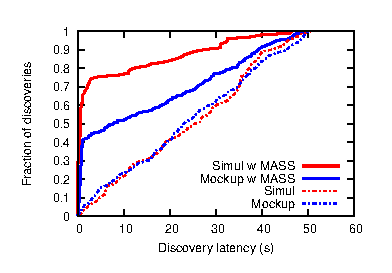
\includegraphics{graphs/latency-mockup/latency-reduction}
   \caption{Discovery latency reduction in mock-up scenario at 1\% duty cycle and 5 ms slot size.}
   \label{fig:latency-reduction}
\end{figure}

In this section, we investigate how much gains can be obtained in discovery latency reduction with
MASS. As comparison, we run the experiments with and without MASS. Firstly, we make the volunteers
carry listening nodes and mobile nodes without MASS and then with MASS following the same randomly
produced traces. We also run the simulator with the same traces for comparison.

Fig.~\ref{fig:latency-reduction} shows the cumulative distribution of the discovery latency in the
mock-up scenario compared with the simulation results. Two observations can be obtained from the
results. The first is that MASS can reduce the discovery latency in the mock-up scenario. Discovery
latency can be reduced to 1~s in 45\% cases. The second observation is that there is a performance
gap between the simualtion result and the result in the practical mock-up scenario. The gap may be
caused by the accuracy of clock skew estimation and clock drift compensation which may break the
slot index synchronization. In practice, the clock skew may change with the environment such as the 
temperature. And the clock drift error will be accumulated if the synchronization can not be updated 
frequently. Thus, it remains the future work to investigate how to improve the synchronization accuracy 
in the real large scale sensor networks.

\section{Conclusion}
\label{sec:conclusion}

In this paper, we show that slot index synchronization is a practical
technique that can significantly improve the average-case performance
of deterministic neighbor discovery protocols. By exploiting the
mobility pattern of the mobile nodes in \emph{docking} applications,
we developed MASS, a reference-based slot index synchronization
technique, that can improve the average discovery latency, while
keeping the energy consumption constant.  We showed with simulations
based on real traces and experiments in a mock-up scenario, that MASS 
can improve the average discovery latency by up to 2 orders of magnitude. 
Our work represents a preliminary investigation into improving existing 
deterministic neighbor discovery protocols by introducing slot index
synchronization. It remains as future work to thoroughly investigate
how MASS will perform on real large scale sensor networks.



%\balance
\bibliographystyle{fitee}
\bibliography{bibsample}

%=========================================
%Authors can choose to use the bibliography or
%directly paste the references beginning with '\item' with the following setting.
%=========================================

%\vspace{9pt} {\par
%\noindent\bf References \par}
%\begin{description}\footnotesize
%
%%{description}
%%\baselineskip 0pt -- line space within an item
%%\itemsep -3pt     -- line space between two items
%
%\itemsep -3.5pt
%
%%\setlength\baselineskip{12pt}
%\makeatletter \setlength{\labelwidth}{0pt}\setlength{\labelsep}{0pt}
%\renewenvironment{thebibliography}[1]
%{\section*{\refname}%
%\@mkboth{\MakeUppercase\refname}{\MakeUppercase\refname}%
%\list{\@biblabel{\@arabic\c@enumiv}}%
%{\settowidth\labelwidth{\@biblabel{#1}}%
%\leftmargin\labelwidth \advance\leftmargin\labelsep
%\advance\leftmargin by 2em %%
%\itemindent -2em %%
%\@openbib@code
%\usecounter{enumiv}%
%\let\p@enumiv\@empty
%\renewcommand\theenumiv{\@arabic\c@enumiv}}%
%\sloppy \clubpenalty4000 \@clubpenalty \clubpenalty
%\widowpenalty4000%
%\sfcode`\.\@m} {\def\@noitemerr
%{\@latex@warning{Empty `thebibliography' environment}}%
%\endlist}
%\makeatother
%
%\vspace{-9pt}
%
%\item  Cookson, A.H., 1985. Particle Trap for Compressed Gas Insulated Transmission Systems. US Patent, 4554399.
%\item  Deniz, O., Castrillon, M., Lorenzo, J., Anton, L., Hernandez, M., Bueno, G., 2010. Computer vision based eyewear selector. {\em J. Zhejiang Univ.-Sci. C (Comput. \& Electron.)}, {\bf11}(2):79--91. [doi:10.1631/jzus.C0910377]
%\item  Gorini, S., Quirini, M., Menciassi, A., Permorio, G., Stefanini, C., Dario, P., 2006. A Novel SMA-Based Actuator for a Legged Endoscopic Capsule. First IEEE/RAS-EMBS International Conference on Biomedical Robotics and Biomechatronics, p.443--449. [doi:10.1109/BIOROB.2006.1639128]
%\item  Gregersen, H., 2006. Biomechanics of the Gastrointestinal Tract. People's Medical Publishing House, Beijing, China, p.216--236.
%\item  ISO 4948-1:1982. Steels-Classification-Part 1: Classification of Steels into Unalloyed and Alloy Steels Based on Chemical Composition. International Organization for Standardization, Geneva.
%\item  Kampf, S.K., Salazar, M., Tyler, S.W., 2002. Preliminary investigations of effluent drainage from mining heap leach facilities. \emph{Vadose Zone J.}, \textbf{1}(1):186--196. Available from http://www.vadosezonejournal.org
%\item  Prigogine, I., 1976. Order Through Fluctuation: Self Organization and Social System. \emph{In}: Jantsch, E., Waddington, C. (Eds.), Evolution and Consciousness: Human Systems in Transition. Addison-Wesley, London, p.93--134.
%\item  RedHat, Microsoft, IBM and Sun, 2010. A Hand Book for Computers. ebook series 1(1):1--1000. Available from http://www.opticalinnovations.com
%\item  Rizvi, U.H., 2006. Combined Multiple Transmit Antennas and Multi-Level Modulation Techniques. MS Thesis, Royal Institute of Technology, Stockholm, Sweden (in Swedish).
%\item  Sweeney, L., 2000. Uniqueness of Simple Demographics in the U.S. Population. Technical Report, No.~LIDAP-WP4. Laboratory for International Data Privacy, Carnegie Mellon University, PA.
%\item  Tanner, N.A., Wait, J.R., Farrar, C.R., Sohn, H., 2003. Structural health monitoring using modular wireless sensors. \emph{J. Intell. Mater. Syst. Struct.}, \textbf{14}(1):43--56. [doi:10.1177/1045389X03014001005]
%\item  Theodoridis, D., Boutalis, Y., Christodoulou, M., 2011. Direct adaptive regulation of unknown nonlinear systems with analysis of the model order problem. {\em J. Zhejiang Univ.-Sci. C (Comput. \& Electron.)}, {\bf12}(1):1--16. [doi:10.1631/jzus.C1000224]
%\item  University of Sheffield Library, 2001. Citing Electronic Sources of Information. Available from http://www.shef.ac.uk/library/libdocs/hsldvc1.pdf [Accessed on Feb. 23, 2007].
%\item  Wu, Z., An, Y., Wang, Z., Yang, S., Chen, H., Zhou, Z., Mai, S., 2008. Study on zoelite enhanced contact adsorption regeneration-stabilization process for nitrogen removal. \emph{J. Hazard. Mater.}, in press. [doi:10.1016/j.jhazmat.2007.12.029]
%\item  Xu, H.H., Zhu, J., 2011. An iterative approach to bayes risk decoding and system combination. {\em J. Zhejiang Univ.-Sci. C (Comput. \& Electron.)}, {\bf12}(3):204--212. [doi:10.1631/jzus.C1000045]
%\item  Yu, L., Wang, J.P., 2010. Review of the current and future technologies for video compression. \emph{J. Zhejiang Univ.-Sci. C (Comput. {\sf \slshape \&} Electron.)}, \textbf{11}(1):1--13. [doi:10.1631/jzus.C0910684]
%\item  Zhou, X.C., SHEN, H.B., YE, J.P., 2011. Integrating outlier filtering in large margin training. {\em J. Zhejiang Univ.-Sci. C (Comput. \& Electron.)}, {\bf12}(5):362--370. [doi:10.1631/jzus.C1000361]
%
%\end{description}


\end{document}
